11. а) Подставим координаты точки $A$ в уравнение: $1196=239k+1,\ k=5.$ Построим график прямой $y=5x+1$ по двум точкам $(0;1)$ и $(1;6).$
$$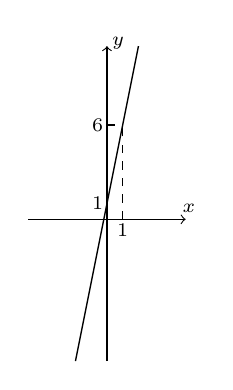
\begin{tikzpicture}[scale=0.2]
\tikzset {line01/.style={line width =0.5pt}}
\tikzset{line02/.style={line width =1pt}}
\tikzset{line03/.style={dashed,line width =0.5pt}}
%\filldraw [black] (0,0) circle (1pt);
\draw [->] (-5,0) -- (5,0);
\draw [->] (0,-9) -- (0,11);
\draw[line01] (-2,-9) -- (2,11);
\draw[line03] (1,0) -- (1,6);
\draw[line03] (0,6) -- (1,6);
\draw (5.2,0.7) node {\scriptsize $x$};
\draw (-0.6,1) node {\scriptsize $1$};
\draw (-0.6,6) node {\scriptsize $6$};
\draw (1,-0.7) node {\scriptsize $1$};
\draw (0.7,11.2) node {\scriptsize $y$};
\end{tikzpicture}$$
б) Эта прямая при любом $k$ проходит через точку $(0;1),$ то есть один из катетов отсекаемого прямоугольного треугольника равен 1. Если второй катет отличается от него в 5 раз, то возможны 4 случая: он больше в 5 раз и точка пересечения с осью абсцисс имеет положительное или отрицательное значение или он меньше в 5 раз и точка пересечения с осью абсцисс имеет положительное или отрицательное значение. Таким образом, искомая прямая должна проходить через одну из точек $(5;0),\ (-5;0),\ \left(\cfrac{1}{5};0\right),\ \left(-\cfrac{1}{5};0\right).$ Подставим эти точки в уравнение прямой и найдём все возможные значения $k:\ 5k+1=0,\ k=-\cfrac{1}{5};\ -5k+1=0,\ k=\cfrac{1}{5};\ \cfrac{1}{5}k+1=0,\ k=-5;\ -\cfrac{1}{5}k+1=0,\ k=5.$\\
